\section{Smart Darts}\label{sec:SmartDarts}

\subsection{Design}

\subsection{Experiments}
\subsubsection{Exp 1: Drop tests in different soils} 
Drop tests as function of soil type, depth and angle\\
\begin{figure} \centering
{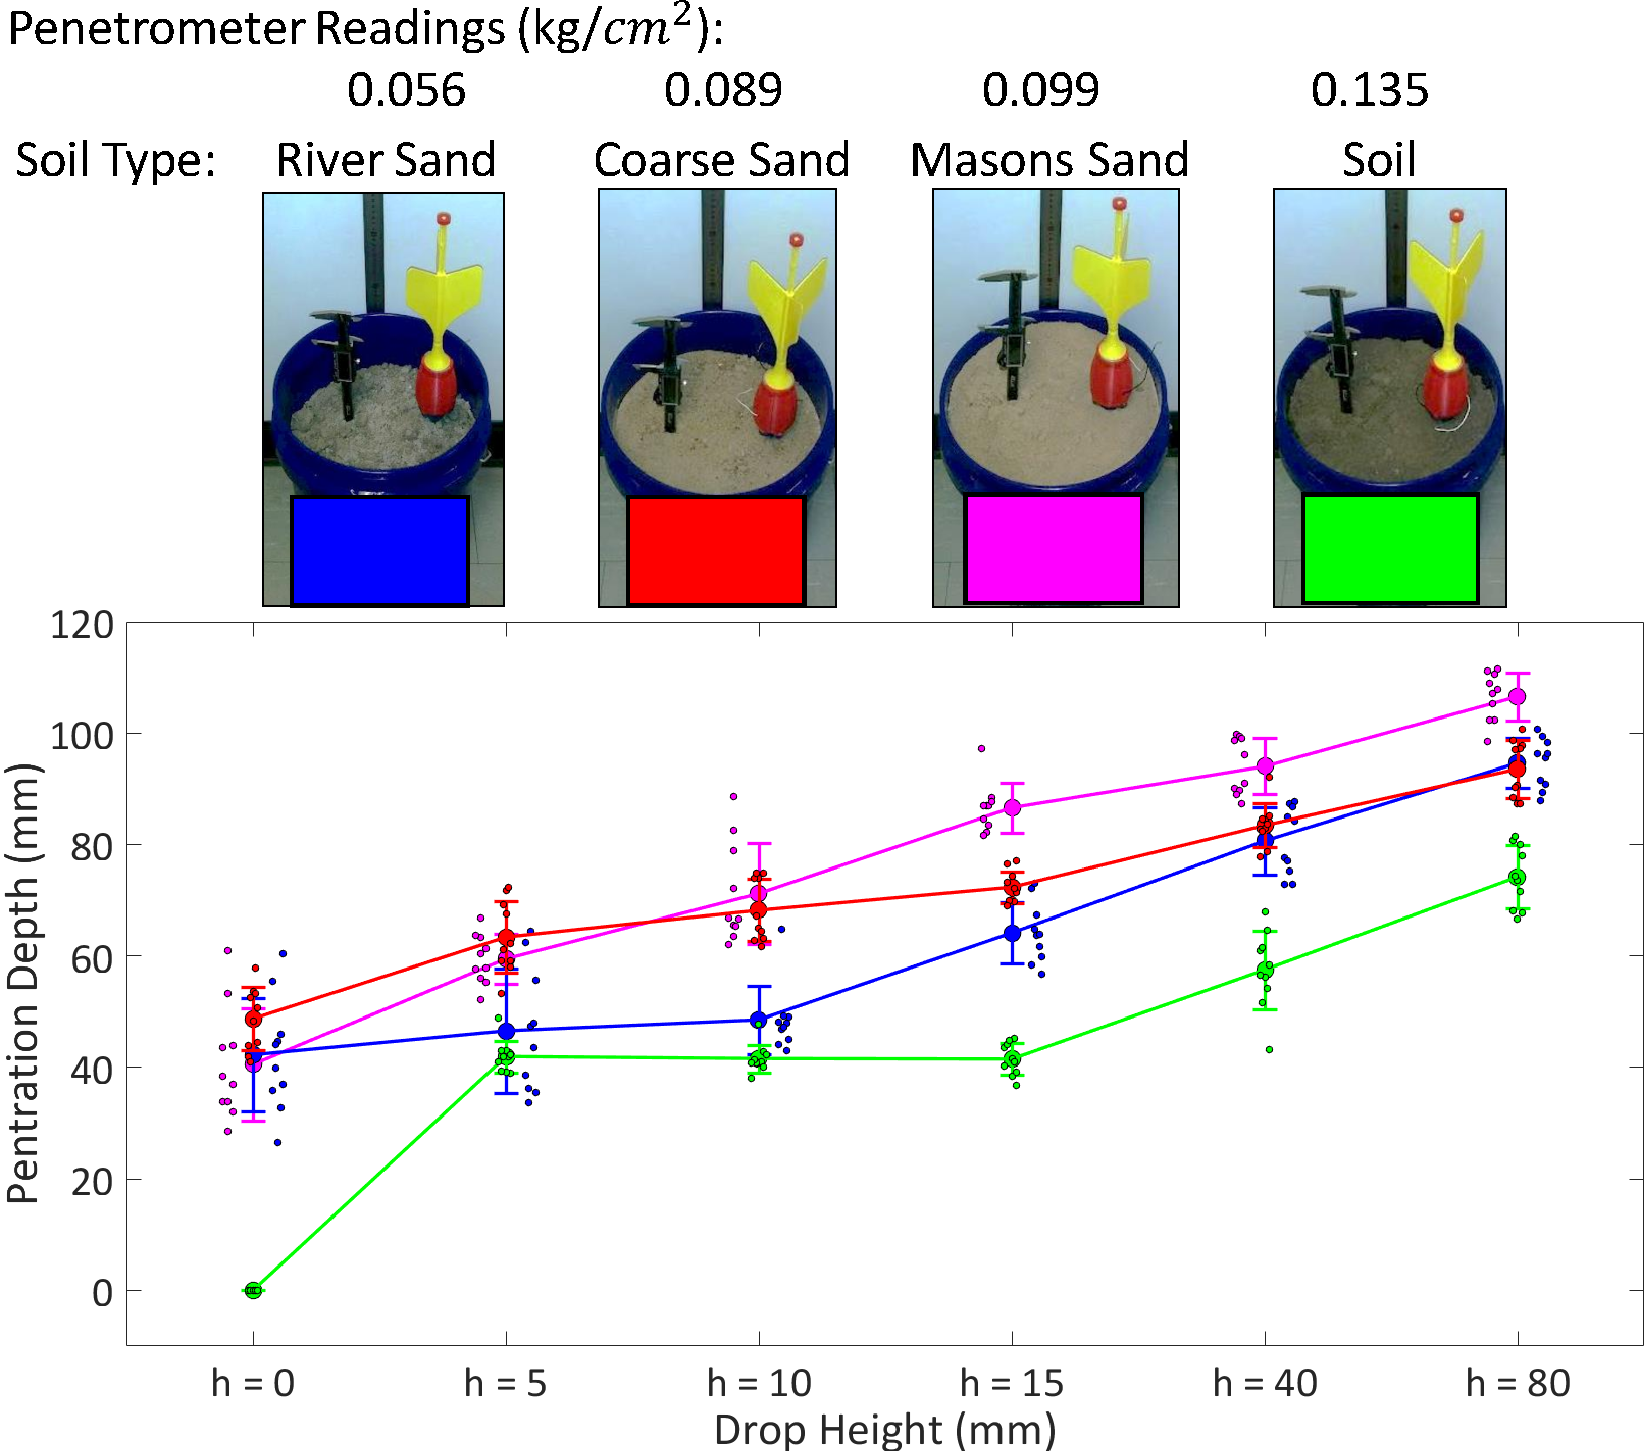
\includegraphics[width=\columnwidth]{indoor_depth_plot.pdf}}
\caption{Drop height vs. penetration depth in four soil types.} 
\label{fig:DepthPlotIndoors}
\vspace{-1em}
\end{figure}
\begin{figure} \centering
{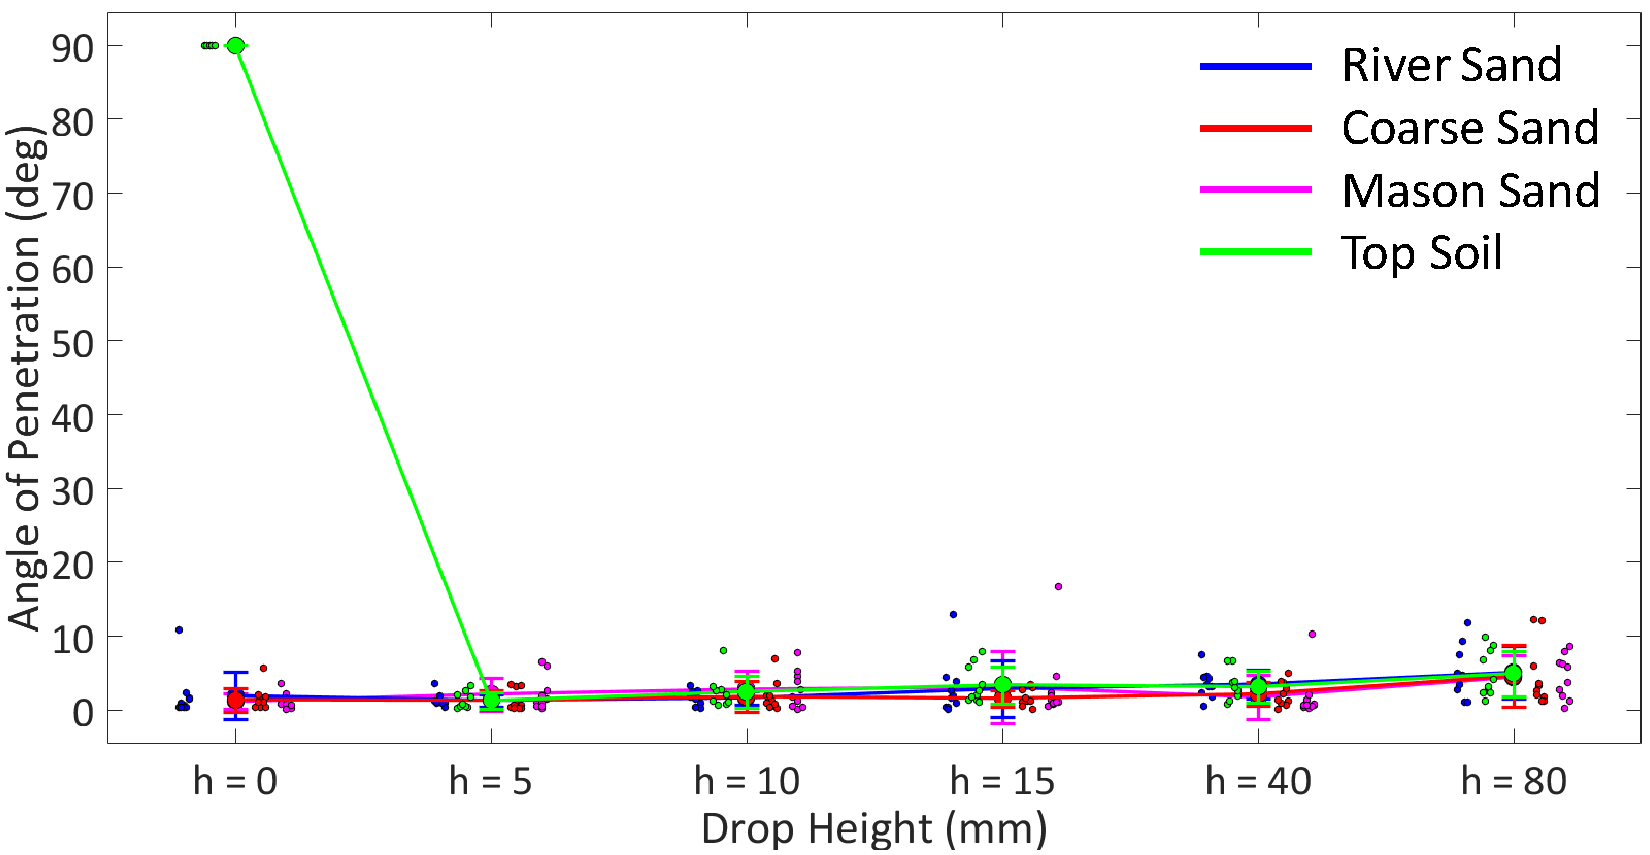
\includegraphics[width=\columnwidth]{indoor_angle_plot.pdf}}
\caption{Drop height vs. angle of deviation in four soil types.} 
\label{fig:AnglePlotIndoors}
\vspace{-1em}
\end{figure}
\subsubsection{Exp 2: Straight vs Bent Fins}
Drop tests as function of height. Compares depth and angle for twisted vs. straight tail.\\
\begin{figure} \centering
  {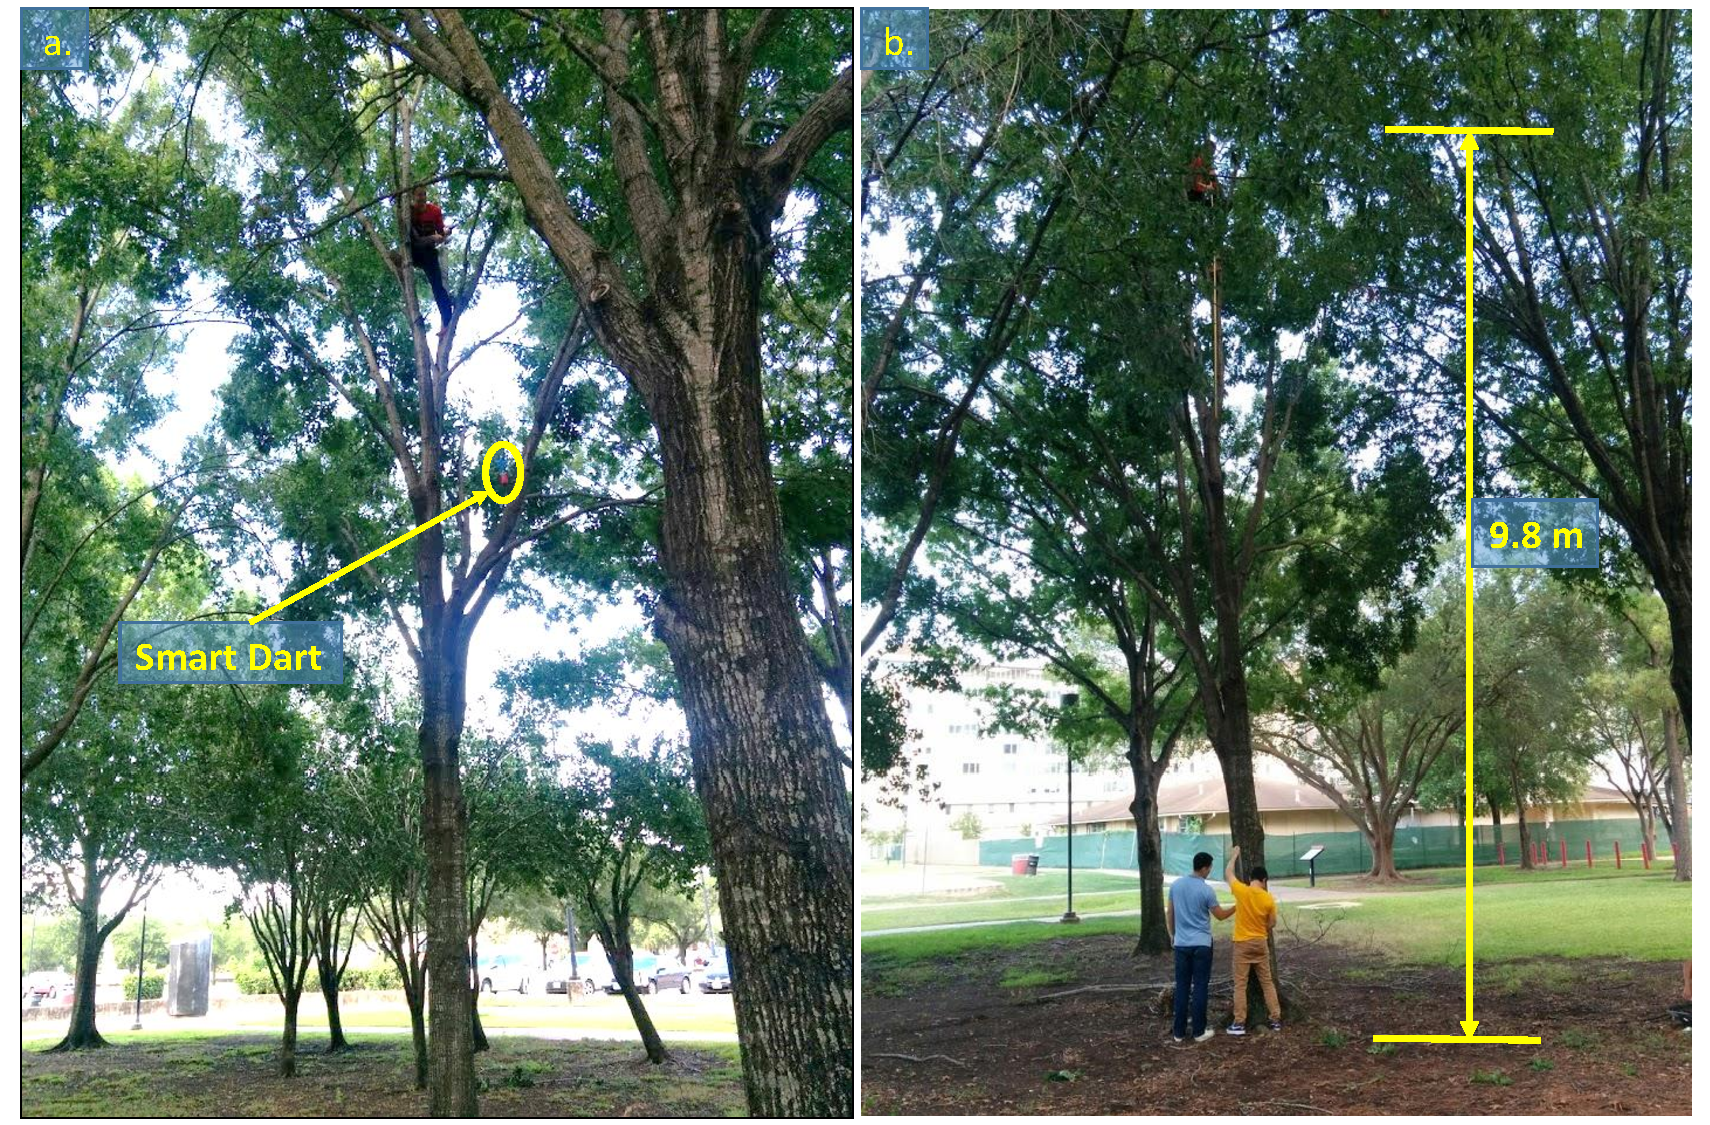
\includegraphics[width=\columnwidth]{StraightBentPic.pdf}}
 \caption{Outdoor Drop test comparing Straight vs Bent fins performance.
 a.)  smart dart dropping 
 b.)  measuring drop height} 
 \label{fig:StraightBentPic}
 \vspace{-1em}
\end{figure}
\begin{figure} \centering
  {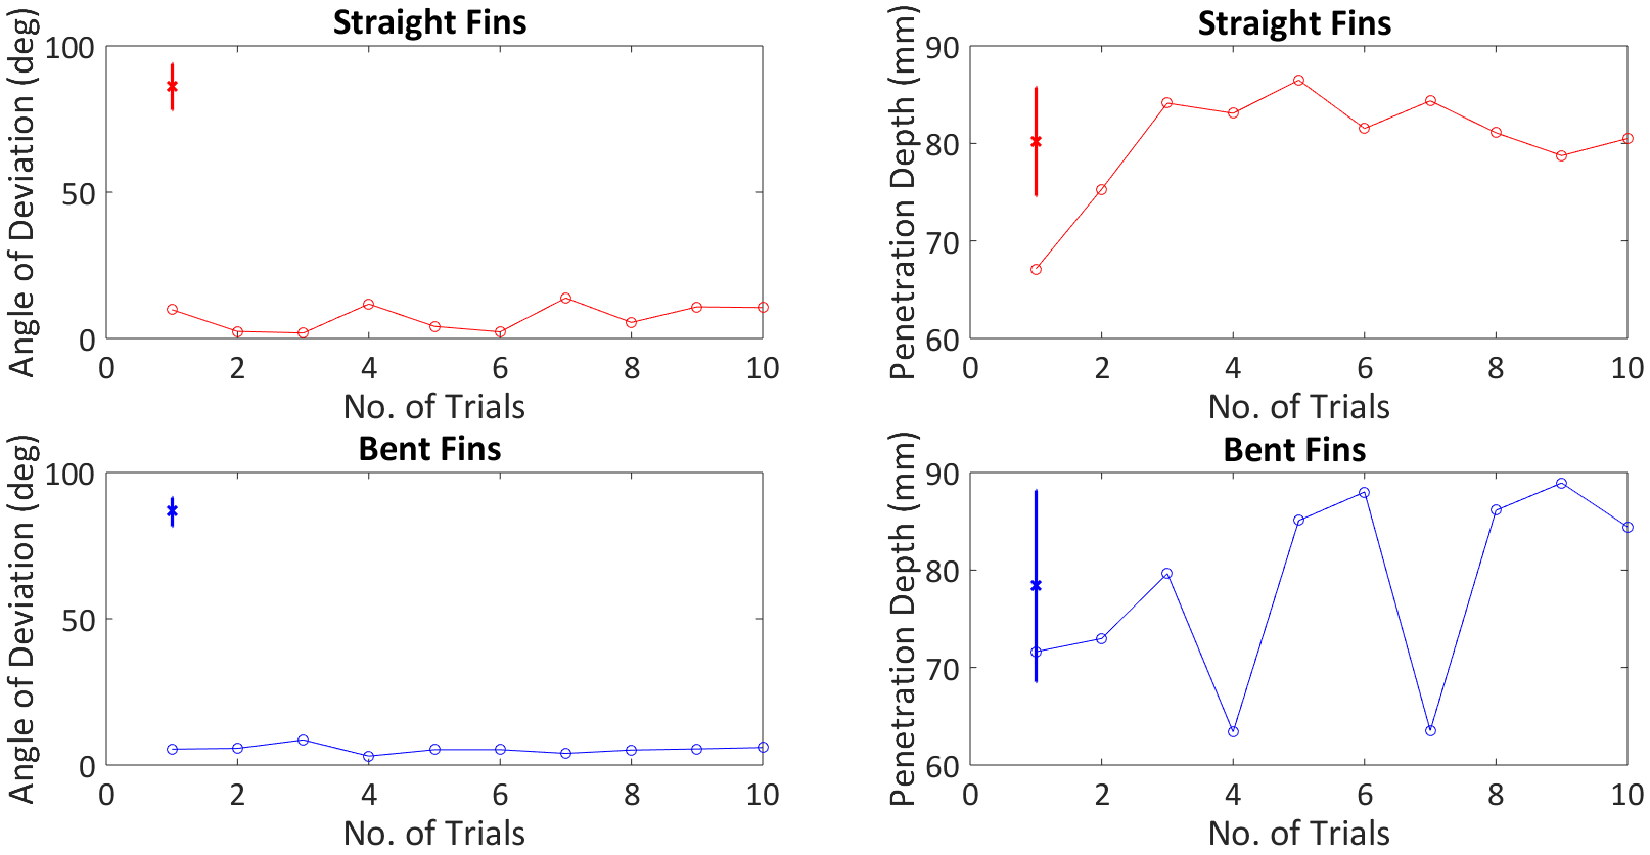
\includegraphics[width=\columnwidth]{StraightBentPlot.pdf}}
 \caption{Straight vs Bent fins comparing penetration depth and angle of deviation. Experiment used a fixed drop height of 9.8 m.} 
 \label{fig:StraightBentPlot}
 \vspace{-1em}
\end{figure}

\subsubsection{Exp 3: Autonomous drop}
Exp 3: Automatic drop from drone, accuracy in placement\\
\subsubsection{Exp 4: Shot gather comparison}
Exp 4: Dart sensing accuracy vs ground setup\\
 